\documentclass[ngerman,openany, oneside]{Script}
\usepackage{amsmath}


% Aufgabentext ein-/ausschalten
\newboolean{aufgabentext}
\setboolean{aufgabentext}{true}
\newcommand{\aufgabentext}[1]{\ifthenelse{\boolean{aufgabentext}}{#1}{}}

% Wenn aufgabentext auch true ist, dann wird der Lösungstext etwas abgesetzt und kursiv geschrieben
\newboolean{mitloesung}
\setboolean{mitloesung}{false}
\newcommand{\loesung}[1]{\ifthenelse{\boolean{mitloesung}}{\ifthenelse{\boolean{aufgabentext}}{{~\\\itshape{#1}}}{#1}}{}}

% Für die Strukturierung
\newcommand{\Thema}[1]{\chapter{#1}}
\newcommand{\Thementeil}[1]{\section{#1}}
\newcommand{\Aufgabe}[1]{\subsection{#1}}
\newcommand{\Unteraufgabe}[1]{\subsubsection{#1}}
\newcommand{\Lernziele}[1]{\subsection*{Lernziele}{#1}}
\graphicspath{{./Bilder/}}

\newcommand{\mucho}[8]{
	\aufgabentext{
	\begin{enumerate}
	\item[#1] \emph{\textbf{#2}} #3
		\begin{enumerate}
		\itemsep1pt\parskip0pt\parsep0pt
		\item[A] #4
		\item[B] #5
		\item[C] #6
		\item[D] #7
		\loesung{Lösung: #8}
		\end{enumerate}
	\end{enumerate}
	}}

\begin{document}

\titelseite[Christian Stoll\\ Sebastian Lange]{Das Praxisskript }%
	{für den Amateurfunkkurs Klasse A}%
	{SoSe 2016}%

\newpage
\thispagestyle{empty}

\begin{tabular}{p{13cm} p{1cm}}
\textbf{Impressum} &\\
&\\
Titel: Praxisskript der Projektwerkstatt DK0TU&\\
Autor: Christian Stoll&\\
1. Auflage Juni 2016 &\\
&\\
Erschienen im :&\\
Fachgebiet Hochfrequenztechnik &\\
Institut für Hochfrequenz- und Halbleiter-Systemtechnologien&\\
Fakultät IV - Elektrotechnik und Informatik &\\
Sekr. HFT 4 &\\
Raum HFT 307 &\\
Einsteinufer 25 &\\
D-10587 Berlin &\\
&\\
Leitung: Prof. Dr. Klaus Petermann &\\
&\\
&\\
%Abbildung:&\\
&\\
Aktuelle Informationen der Projektwerkstatt finden Sie unter:  &\\
\url{http://www.dk0tu.de} &\\
&\\
Die vorliegende Fassung des Praxisskripts wurde sorgfältigst auf Fehler hin überprüft. Um das Praxisskript dennoch laufend verbessern zu können, würden wir uns über Hinweise auf etwaig vorhandene Fehler sowie Verbesserungsvorschläge sehr freuen. Wenden Sie sich dazu bitte an die Tutor\_innen und wissenschaftlichen Mitarbeiter\_innen der Projektwerkstatt. &\\
\end{tabular}




\newpage
%%Inhaltsverzeichnis
\tableofcontents
\newpage

\newpage

\chapter{Der Widerstand}
\begin{wrapfigure}[0]{r}[-1cm]{3cm}
 \vspace{-5cm}
 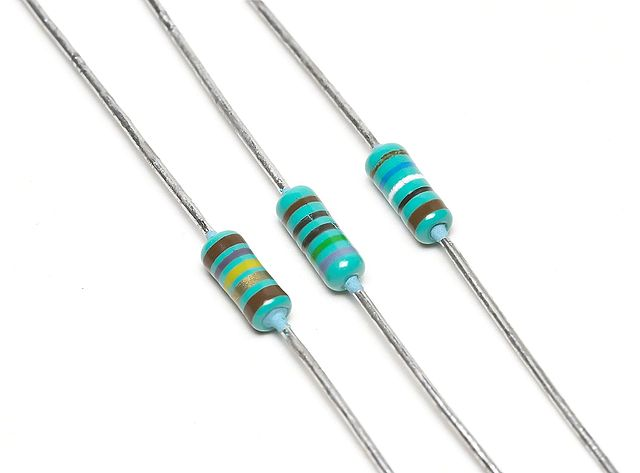
\includegraphics[scale=0.9]{Widerstand/Bilder/Resistors.jpg}
 \vspace{-5cm}
\end{wrapfigure}

\section*{Theorie- und Prüfungsfragen} 

\aufgabentext{
	\begin{enumerate}
	\item[1] \emph{\textbf{TB102}} Welchen Widerstand hat eine Kupferdrahtwicklung, wenn der verwendete Draht eine Länge von 1,8 m und einen Durchmesser von 0,2 mm hat
		\begin{enumerate}
		\itemsep1pt\parskip0pt\parsep0pt
		\item[A] 0,05 $\Omega$
		\item[B] 1 $\Omega$
		\item[C] 5,6 $\Omega$
		\item[D] 56 $\Omega$
		\loesung{Lösung: B}
		\end{enumerate}
	\end{enumerate}
}

\aufgabentext{
	\begin{enumerate}
	\item[2] \emph{\textbf{TC315}} Was verstehen Sie unter dem technischen Ausdruck Skin-Effekt?
		\begin{enumerate}
		\itemsep1pt\parskip0pt\parsep0pt
		\item[A] Als Skin-Effekt bezeichnet man die Erscheinung, dass sich mit steigender Frequenz der Elektronenstrom mehr und mehr zu den Kanten eines Kondensators hin verlagert. Dadurch erhöht sich mit steigender Frequenz die Kapazität.
		\item[B] Als Skin-Effekt bezeichnet man die Erscheinung, dass sich mit steigender Frequenz der Elektronenstrom mehr und mehr zur Oberfläche eines Leiters hin verlagert. Dadurch erhöht sich mit steigender Frequenz der Leiterwiderstand.
		\item[C] Als Skin-Effekt bezeichnet man die Erscheinung, dass sich mit steigender Frequenz die Induktivität und die Kapazität eines Leiters erhöht. Dadurch erhöht sich mit steigendem Leiterwiderstand die Resonanzfrequenz.
		\item[D] Als Skin-Effekt bezeichnet man die Erscheinung, dass sich mit steigender Frequenz der Elektronenstrom mehr und mehr zur Leitermitte hin verlagert. Dadurch erhöht sich der Leiterwiderstand bei hohem Wechselstromanteil.
		\loesung{Lösung: B}
		\end{enumerate}
	\end{enumerate}
}

\mucho{3}{TC102}
{Metallschichtwiderstände}
{haben geringe Fertigungstoleranzen und Temperaturabhängigkeit und sind besonders als Präzisionswiderstände geeignet.}
{sind induktionsarm und eignen sich besonders für den Einsatz bei sehr hohen Frequenzen.}
{sind besonders als Hochlastwiderstände bei niedrigen Frequenzen geeignet.}
{haben einen extrem stark negativen Temperaturkoeffizienten und sind besonders als NTC-Widerstände (Heißleiter) geeignet.}
{A}

\mucho{4}{TC103}
{Metalloxidwiderstände}%Frage
{haben geringe Toleranzen und Widerstandsänderungen und sind besonders als Präzisionswiderstände in der Messtechnik geeignet.}%A
{sind besonders als Hochlastwiderstände bei niedrigen Frequenzen geeignet.}%B
{sind induktionsarm und eignen sich besonders für den Einsatz bei sehr hohen Frequenzen.}%C
{haben einen extrem stark negativen Temperaturkoeffizienten und sind besonders als NTC-Widerstände (Heißleiter) geeignet.}%D
{C}%Lösung

\mucho{5}{TC104}
{Drahtwiderstände}%Frage
{Drahtwiderstände werden hauptsächlich in Form von SMD-Widerständen hergestellt.}%A
{sind induktionsarm und eignen sich besonders für den Einsatz bei sehr hohen Frequenzen.}%B
{haben einen extrem stark negativen Temperaturkoeffizienten und sind besonders als NTC-Widerstände (Heißleiter) geeignet.}%C
{sind besonders als Hochlastwiderstände bei niedrigen Frequenzen geeignet.}%D
{D}%Lösung

\mucho{6}{TB202}
{Die Leerlaufspannung  einer Gleichspannungsquelle beträgt 13,5 V. Wenn die Spannungsquelle einen Strom von 0,9 A abgibt, sinkt die Klemmenspannung auf 12,4 V. Wie groß ist der Innenwiderstand der Spannungsquelle?}%Frage
{0,82$\Omega$}%A
{1,1$\Omega$}%B
{1,22 $\Omega$}%C
{12,15 $\Omega$}%D
{C}%Lösung

\mucho{7}{TB204}
{Die Leerlaufspannung einer Gleichspannungsquelle beträgt 13,5 V. Wenn die Spannungsquelle einen Strom von 1 A abgibt, sinkt die Klemmenspannung auf 12,5 V. Wie groß ist der Wirkungsgrad der Spannungsquelle?}%Frage
{7,5 $\%$}%A
{13,5 $\%$}%B
{92,6 $\%$}%C
{100 $\%$}%D
{C}%Lösung

\mucho{8}{TB207}
{In welchem Zusammenhang müssen Innenwiderstand Ri und Lastwiderstand RL stehen, damit Leistungsanpassung vorliegt?}%Frage
{$R_L = R_i$}%A
{$R_L >> R_i$}%B
{$R_L << R_i$}%C
{$R_L = 1/R_i$}%D
{A}%Lösung

\mucho{9}{TB209}
{In welchem Zusammenhang müssen Innenwiderstand Ri und Lastwiderstand RL stehen, damit Spannungsanpassung vorliegt?}%Frage
{$R_L = R_i$}%A
{$R_L >> R_i$}%B
{$R_L << R_i$}%C
{$R_L = 1/R_i$}%D
{B}%Lösung

\mucho{10}{TB208}
{In welchem Zusammenhang müssen Innenwiderstand Ri und Lastwiderstand RL stehen, damit Stromanpassung vorliegt?}%Frage
{$R_L = R_i$}%A
{$R_L >> R_i$}%B
{$R_L << R_i$}%C
{$R_L = 1/R_i$}%D
{C}%Lösung

\chapter{Der Kondensator und die Spule}
\begin{wrapfigure}[0]{r}[-2.5cm]{3cm}
 \vspace{-6cm}
 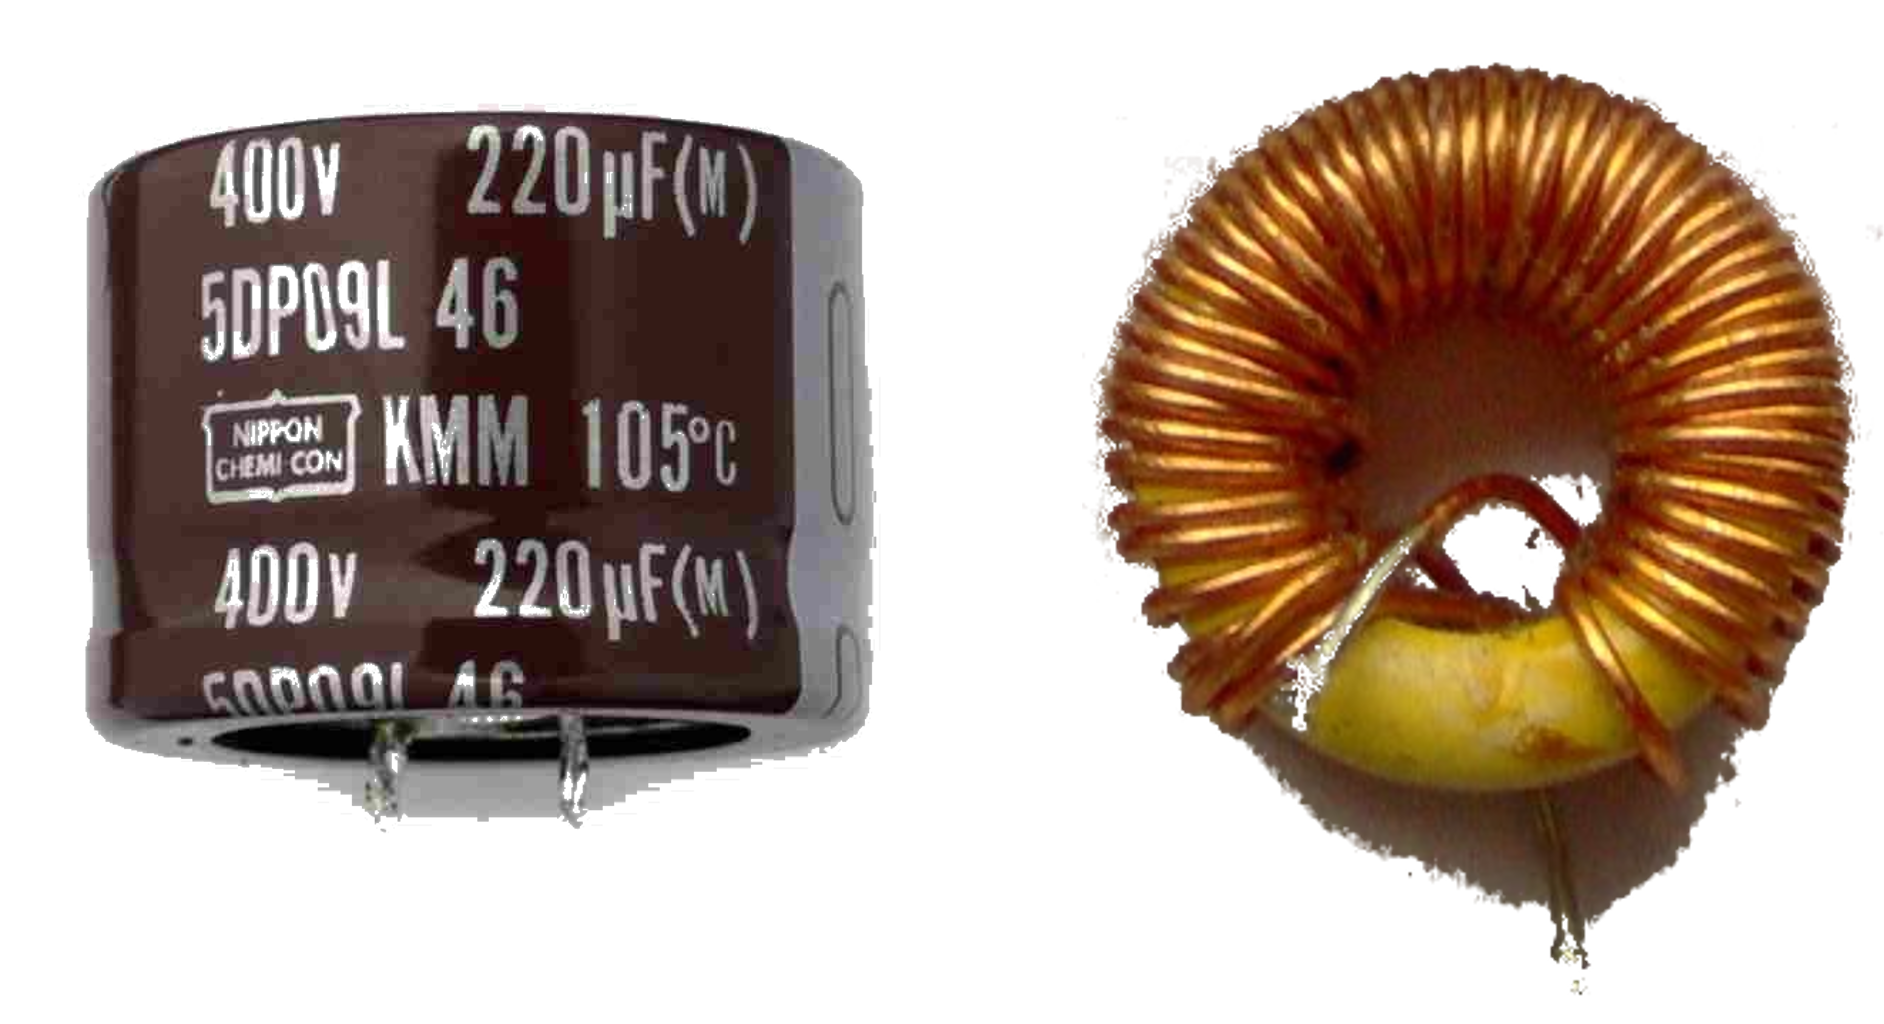
\includegraphics[scale=0.4]{KondensatorSpule/Bilder/KondensatorSpule.png}
 \vspace{-6cm}
\end{wrapfigure}

\section*{Theorie- und Prüfungsfragen} 


\mucho{1}{TC204}
{Wie verhält sich der Wechselstromwiderstand eines Kondensators mit zunehmender Frequenz?}%Frage
{Er bleibt konstant.}%A
{Er nimmt zu.}%B
{Er nimmt ab.}%C
{Er wird unendlich.}%D
{C}%Lösung

\mucho{2}{TC205}
{Wie groß ist der kapazitive Widerstand eines 10-pF-Kondensators bei 100 MHz?}%Frage
{31,8 $\Omega$}%A
{159 $\Omega$}%B
{318 $\Omega$}%C
{1,58 $k\Omega$}%D
{B}%Lösung

\mucho{3}{TC203}
{Ein verlustloser Kondensator wird an eine Wechselspannungsquelle angeschlossen. Welche Phasenverschiebung zwischen Spannung und Strom stellt sich ein?}%Frage
{Die Spannung eilt dem Strom um 45$^\circ$ voraus.}%A
{Der Strom eilt der Spannung um 45$^\circ$ voraus.}%B
{Der Strom eilt der Spannung um 90$^\circ$ voraus.}%C
{Die Spannung eilt dem Strom um 90$^\circ$ voraus.
}%D
{C}%Lösung

\mucho{4}{TC207}
{Was versteht man unter dem Blindwiderstand eines Kondensators und von welchen physikalischen Größen hängt er ab?}%Frage
{Der Blindwiderstand ist der Wechselstromwiderstand eines Kondensators. Er ist abhängig von der Kapazität des Kondensators und der anliegenden Frequenz. Im Blindwiderstand entstehen keine Wärmeverluste.}%A
{Der Blindwiderstand ist der Gleichstromwiderstand eines Kondensators. Er ist abhängig vom Isolationsmaterial des Kondensators und der anliegenden Spannung. Auch im Blindwiderstand entstehen Wärmeverluste.}%B
{Der Blindwiderstand ist der Wechselstromwiderstand eines Kondensators. Er ist abhängig von der Blindkapazität des Kondensators und der anliegenden Spannung. Im Blindwiderstand entstehen hohe Verluste.}%C
{Der Blindwiderstand ist der HF-Gleichstromwiderstand eines Kondensators. Er wird mit steigender Kapazität sowie bei erhöhtem Wechselstromanteil und steigender Frequenz größer. Je höher die Frequenz umso eher wandern die Ladungen an die Plattenränder (Skin-Effekt).}%D
{A}%Lösung

\mucho{5}{TD103}
{Wie groß ist die Gesamtkapazität von drei parallel geschalteten Kondensatoren von 20$nF$, 0,03$\mu F$ und 15000$pF$?}%Frage
{0,650$\mu F$}%A
{650$nF$}%B
{0,065$\mu F$}%C
{650000 $pF$}%D
{C}%Lösung

\mucho{6}{TC310}
{Mit einem Schalenkern, dessen AL-Wert mit 250 angegeben ist, soll eine Spule mit einer Induktivität von 2$mH$ hergestellt werden. Wie groß ist die erforderliche Windungszahl?}%Frage
{3}%A
{53}%B
{89}%C
{2828}%D
{C}%Lösung


\mucho{7}{TC306}
{Was versteht man unter dem Blindwiderstand einer Spule und von welchen physikalischen Größen hängt er ab?}%Frage
{Der Blindwiderstand ist der Wechselstromwiderstand einer Spule. Er ist abhängig von der Induktivität der Spule und der anliegenden Frequenz. Im Blindwiderstand entstehen keine Wärmeverluste.}%A
{Der Blindwiderstand ist der Gleichstromwiderstand einer Spule. Er ist abhängig vom Isolationsmaterial der Spule und der anliegenden Spannung. Auch im Blindwiderstand entstehen Wärmeverluste.}%B
{Der Blindwiderstand ist der Wechselstromwiderstand einer Spule. Er ist abhängig von der Blindinduktivität der Spule und der anliegenden Spannung. Im Blindwiderstand entstehen hohe Verluste.}%C
{Der Blindwiderstand ist der HF-Gleichstromwiderstand einer Spule. Er wird mit steigender Induktivität sowie bei erhöhtem Wechselstromanteil und steigender Frequenz größer. Je tiefer die Frequenz umso eher wandern die Elektronen an den Spulenrand (Skin-Effekt).}%D
{A}%Lösung

\mucho{8}{TC305}
{Wie groß ist der Wechselstromwiderstand einer Spule mit 3$\mu H$ Induktivität bei einer Frequenz von 100 MHz?}%Frage
{1,9$\Omega$}%A
{942$\Omega$}%B
{1885$\Omega$}%C
{1885$k\Omega$}%D
{C}%Lösung

\mucho{9}{TC302}
{In einer reinen Induktivität, die an einer Wechselspannungsquelle angeschlossen ist, eilt der Strom der angelegten Spannung ...}%Frage
{um 90 $^\circ$ voraus.}%A
{um 90 $^\circ$ nach.}%B
{um 45 $^\circ$ voraus.}%C
{um 45 $^\circ$ nach.}%D
{B}%Lösung


\chapter{Die Diode}


\begin{wrapfigure}[0]{r}[-2cm]{4cm}
 \vspace{-5cm}
 %\centering 
 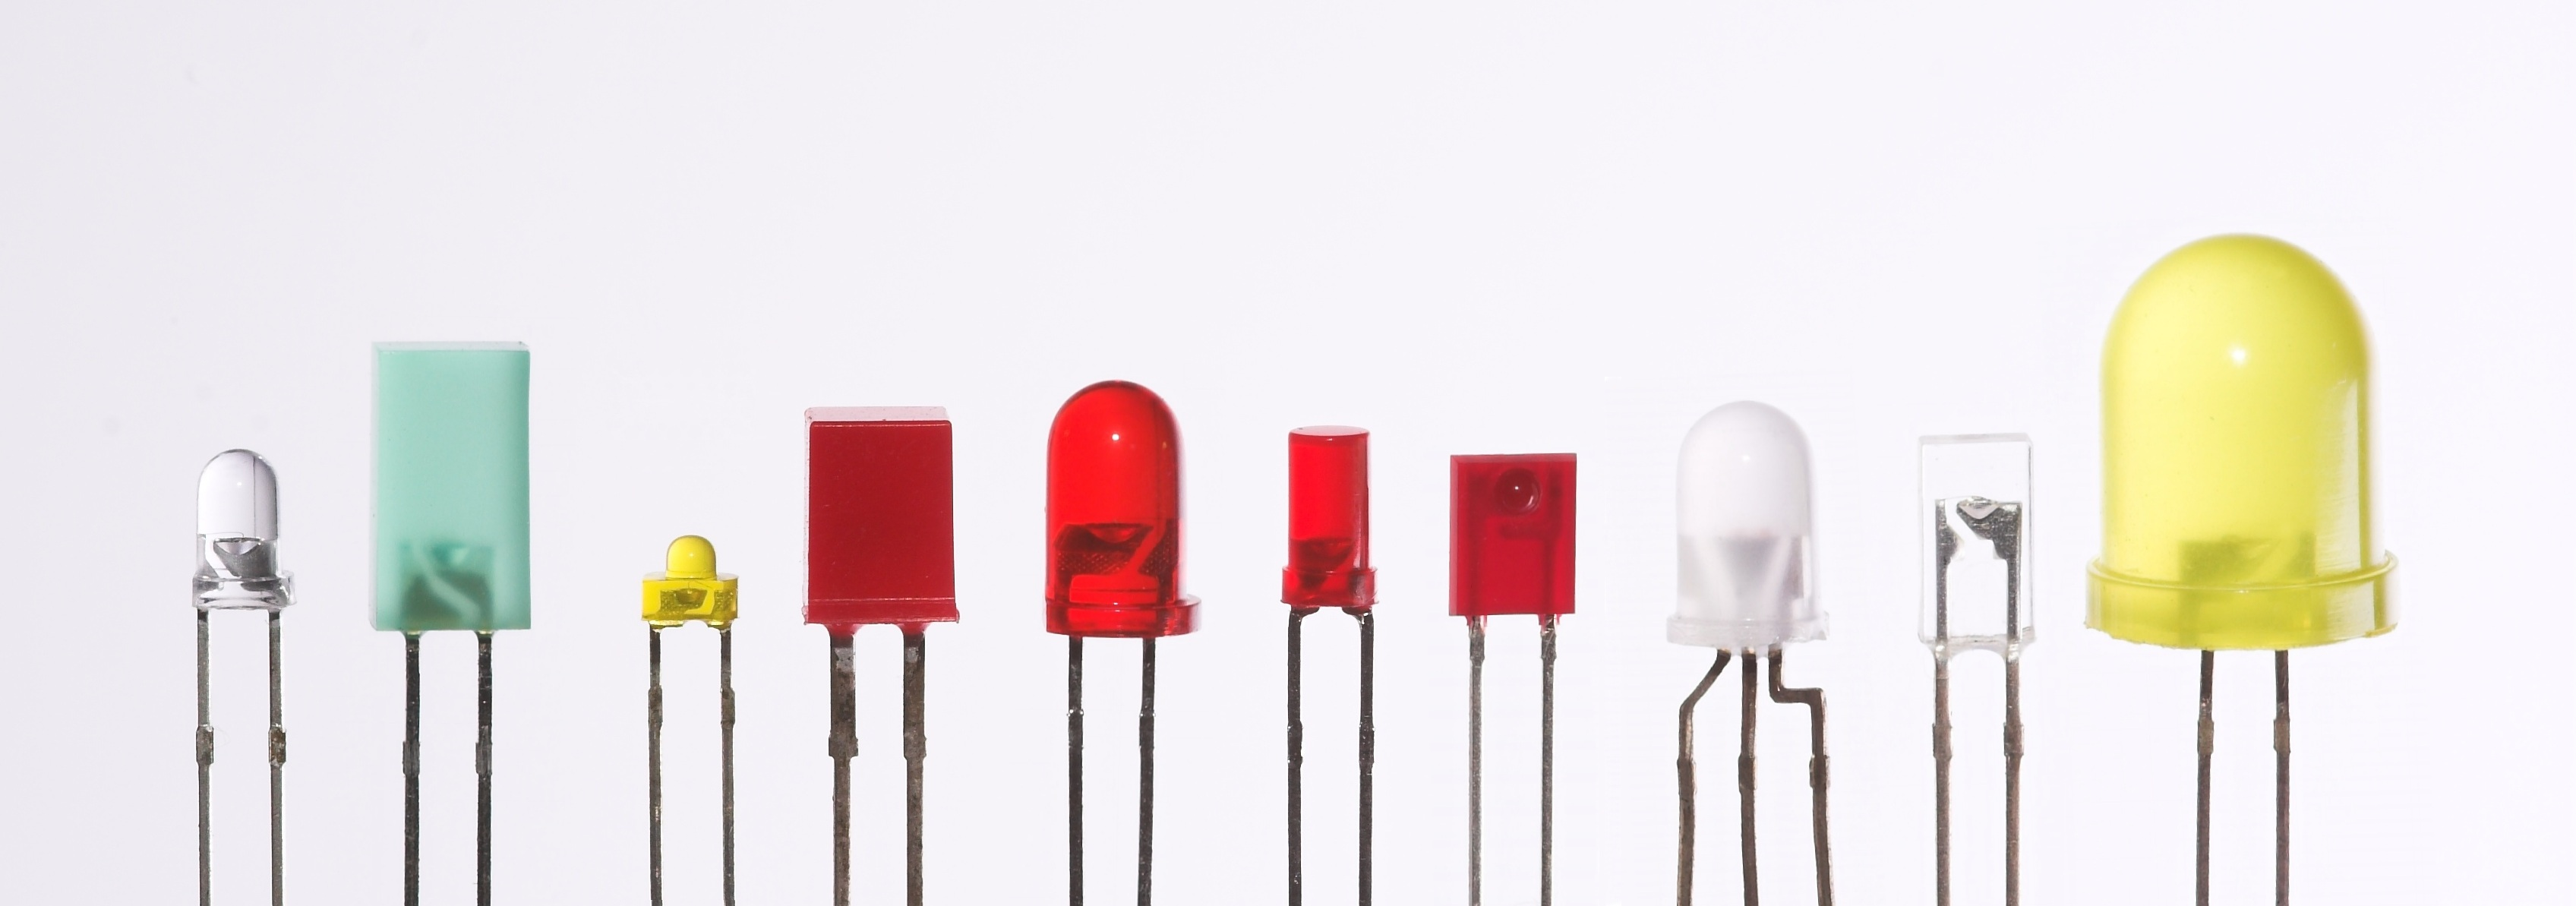
\includegraphics[scale=0.25]{Diode/Bilder/Verschiedene_LEDs.jpg}
 %\caption{Bildunterschrift der Grafik.}
 %\label{fig:meine-Grafik}
 \vspace*{-5cm}
\end{wrapfigure}


\section*{Theorie- und Prüfungsfragen} 

\subsection*{Dotierung}

\begin{enumerate}
	\itemsep1pt\parskip0pt\parsep0pt
	\item[1] Was bedeutet der Begriff Dotierung?
        \loesung{\textbf{Dotierung} bezeichnet in der Halbleitertechnik das
        einbringen von Fremdatomen in ein Grundmaterial zur Veränderung der
        elektrischen Leitfähigkeit.}
\end{enumerate}

\begin{enumerate}
\item[2] \emph{\textbf{TB105}}    Was verstehen Sie unter Halbleitermaterialien? Einige Stoffe wie z.B. ...
	\begin{enumerate}
	\itemsep1pt\parskip0pt\parsep0pt
		\item[A] Silizium, Germanium sind in reinem Zustand gute Isolatoren. Durch geringfügige Zusätze von geeigneten anderen Stoffen werden sie jedoch zu Leitern.
		\item[B] Silizium, Germanium sind in reinem Zustand gute Isolatoren. Durch geringfügige Zusätze von geeigneten anderen Stoffen nimmt jedoch ihre Leitfähigkeit ab.
		\item[C]  Indium oder Magnesium sind in reinem Zustand gute Isolatoren. Durch geringfügige Zusätze von geeigneten anderen Stoffen werden sie jedoch zu Leitern.
		\item[D] Silizium, Germanium sind in trockenem Zustand gute Elektrolyten. Durch geringfügige Zusätze von Wismut oder Tellur kann man daraus entweder N-leitendes oder P-leitendes Material für Anoden bzw. Katoden von Halbleiterbauelementen herstellen.
		\loesung{Lösung A}
	\end{enumerate}
\end{enumerate}

\begin{enumerate}
\item[3] \emph{\textbf{TC501}}    P-dotiertes Halbleitermaterial ist solches, das mit einem zusätzlichen Stoff versehen wurde, der
	\begin{enumerate}
	\itemsep1pt\parskip0pt\parsep0pt
		\item[A] mehr als vier Valenzelektronen enthält.
		\item[B] genau vier Valenzelektronen enthält.
		\item[C] weniger als vier Valenzelektronen enthält.
		\item[D] keine Valenzelektronen enthält.
		 \loesung{Lösung C}
	\end{enumerate}
\end{enumerate}


\begin{enumerate}
\item[4] \emph{\textbf{TC502}}   N-leitendes Halbleitermaterial ist gekennzeichnet durch
	\begin{enumerate}
	\itemsep1pt\parskip0pt\parsep0pt
		\item[A] Überschuss an freien Elektronen.
		\item[B] das Fehlen von Dotierungsatomen.
		\item[C] das Fehlen von Atomen im Gitter des Halbleiterkristalls.
		\item[D] bewegliche Elektronenlücken.
		\loesung{Lösung A}
	\end{enumerate}
\end{enumerate}


\begin{enumerate}
\item[5] \emph{\textbf{TC503}}  Ein in Durchlassrichtung betriebener PN-Übergang ermöglicht
	\begin{enumerate}
	\itemsep1pt\parskip0pt\parsep0pt
		\item[A] den Stromfluss von N nach P.
		\item[B] den Stromfluss von P nach N.
		\item[C] keinen Stromfluss.
		\item[D] den Elektronenfluss von P nach N.
		\loesung{Lösung B}
	\end{enumerate}
\end{enumerate}


\subsection*{Die Diode}

\begin{enumerate}
\itemsep1pt\parskip0pt\parsep0pt
\item[6] Skizziere das Schaltzeichen einer Diode und markiere die Anode, die Kathode und die jeweilige Dotierung.
    \loesung{
    \begin{figure}[H]
    \centering 
    % Graphic for TeX using PGF
% Title: /home/stole/Dokumente/git/afutub-kurs/Praxisskript/Diode/Schaltungen/Diode.dia
% Creator: Dia v0.97.3
% CreationDate: Mon Nov 16 20:36:17 2015
% For: stole
% \usepackage{tikz}
% The following commands are not supported in PSTricks at present
% We define them conditionally, so when they are implemented,
% this pgf file will use them.
\ifx\du\undefined
  \newlength{\du}
\fi
\setlength{\du}{15\unitlength}
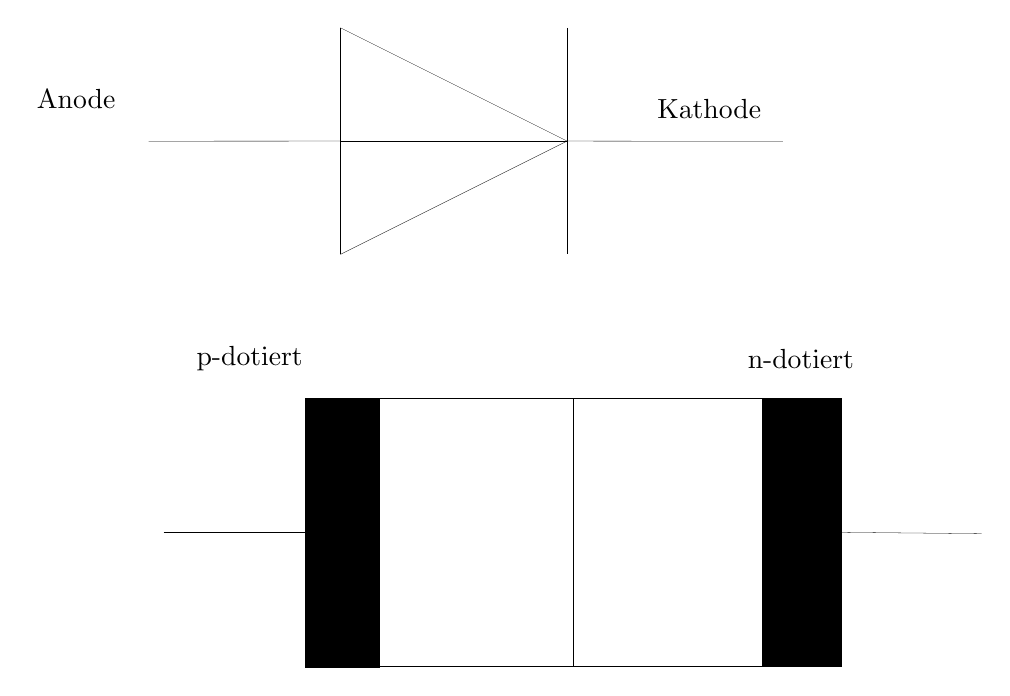
\begin{tikzpicture}
\pgftransformxscale{1.000000}
\pgftransformyscale{-1.000000}
\definecolor{dialinecolor}{rgb}{0.000000, 0.000000, 0.000000}
\pgfsetstrokecolor{dialinecolor}
\definecolor{dialinecolor}{rgb}{1.000000, 1.000000, 1.000000}
\pgfsetfillcolor{dialinecolor}
\pgfsetlinewidth{0.100000\du}
\pgfsetdash{}{0pt}
\pgfsetdash{}{0pt}
\pgfsetbuttcap
\pgfsetmiterjoin
\pgfsetbuttcap
\pgfsetmiterjoin
\pgfsetdash{}{0pt}
\definecolor{dialinecolor}{rgb}{0.000000, 0.000000, 0.000000}
\pgfsetstrokecolor{dialinecolor}
\draw (15.422302\du,-15.899999\du)--(15.422302\du,-13.022298\du);
\pgfsetbuttcap
\pgfsetmiterjoin
\pgfsetdash{}{0pt}
\definecolor{dialinecolor}{rgb}{0.000000, 0.000000, 0.000000}
\pgfsetstrokecolor{dialinecolor}
\draw (15.422302\du,-13.022298\du)--(18.300002\du,-14.461149\du);
\pgfsetbuttcap
\pgfsetmiterjoin
\pgfsetdash{}{0pt}
\definecolor{dialinecolor}{rgb}{0.000000, 0.000000, 0.000000}
\pgfsetstrokecolor{dialinecolor}
\draw (15.422302\du,-15.899999\du)--(18.300002\du,-14.461149\du);
\pgfsetbuttcap
\pgfsetmiterjoin
\pgfsetdash{}{0pt}
\definecolor{dialinecolor}{rgb}{0.000000, 0.000000, 0.000000}
\pgfsetstrokecolor{dialinecolor}
\draw (15.422302\du,-14.461149\du)--(18.300002\du,-14.461149\du);
\pgfsetbuttcap
\pgfsetmiterjoin
\pgfsetdash{}{0pt}
\definecolor{dialinecolor}{rgb}{0.000000, 0.000000, 0.000000}
\pgfsetstrokecolor{dialinecolor}
\draw (18.300002\du,-15.899999\du)--(18.300002\du,-13.022298\du);
\pgfsetlinewidth{0.100000\du}
\pgfsetdash{}{0pt}
\pgfsetdash{}{0pt}
\pgfsetbuttcap
{
\definecolor{dialinecolor}{rgb}{0.000000, 0.000000, 0.000000}
\pgfsetfillcolor{dialinecolor}
% was here!!!
\definecolor{dialinecolor}{rgb}{0.000000, 0.000000, 0.000000}
\pgfsetstrokecolor{dialinecolor}
\draw (18.300002\du,-14.461149\du)--(21.040301\du,-14.459230\du);
}
\pgfsetlinewidth{0.100000\du}
\pgfsetdash{}{0pt}
\pgfsetdash{}{0pt}
\pgfsetbuttcap
{
\definecolor{dialinecolor}{rgb}{0.000000, 0.000000, 0.000000}
\pgfsetfillcolor{dialinecolor}
% was here!!!
\definecolor{dialinecolor}{rgb}{0.000000, 0.000000, 0.000000}
\pgfsetstrokecolor{dialinecolor}
\draw (12.987653\du,-14.460276\du)--(15.422302\du,-14.461149\du);
}
% setfont left to latex
\definecolor{dialinecolor}{rgb}{0.000000, 0.000000, 0.000000}
\pgfsetstrokecolor{dialinecolor}
\node[anchor=west] at (11.448825\du,-14.995418\du){Anode};
% setfont left to latex
\definecolor{dialinecolor}{rgb}{0.000000, 0.000000, 0.000000}
\pgfsetstrokecolor{dialinecolor}
\node[anchor=west] at (19.327825\du,-14.872736\du){Kathode};
\pgfsetlinewidth{0.100000\du}
\pgfsetdash{}{0pt}
\pgfsetdash{}{0pt}
\pgfsetmiterjoin
\definecolor{dialinecolor}{rgb}{1.000000, 1.000000, 1.000000}
\pgfsetfillcolor{dialinecolor}
\fill (14.976770\du,-11.192971\du)--(14.976770\du,-7.792972\du)--(18.376770\du,-7.792972\du)--(18.376770\du,-11.192971\du)--cycle;
\definecolor{dialinecolor}{rgb}{0.000000, 0.000000, 0.000000}
\pgfsetstrokecolor{dialinecolor}
\draw (14.976770\du,-11.192971\du)--(14.976770\du,-7.792972\du)--(18.376770\du,-7.792972\du)--(18.376770\du,-11.192971\du)--cycle;
\pgfsetlinewidth{0.100000\du}
\pgfsetdash{}{0pt}
\pgfsetdash{}{0pt}
\pgfsetmiterjoin
\definecolor{dialinecolor}{rgb}{1.000000, 1.000000, 1.000000}
\pgfsetfillcolor{dialinecolor}
\fill (18.376770\du,-11.192970\du)--(18.376770\du,-7.792971\du)--(21.776770\du,-7.792971\du)--(21.776770\du,-11.192970\du)--cycle;
\definecolor{dialinecolor}{rgb}{0.000000, 0.000000, 0.000000}
\pgfsetstrokecolor{dialinecolor}
\draw (18.376770\du,-11.192970\du)--(18.376770\du,-7.792971\du)--(21.776770\du,-7.792971\du)--(21.776770\du,-11.192970\du)--cycle;
\pgfsetlinewidth{0.100000\du}
\pgfsetdash{}{0pt}
\pgfsetdash{}{0pt}
\pgfsetbuttcap
{
\definecolor{dialinecolor}{rgb}{0.000000, 0.000000, 0.000000}
\pgfsetfillcolor{dialinecolor}
% was here!!!
\definecolor{dialinecolor}{rgb}{0.000000, 0.000000, 0.000000}
\pgfsetstrokecolor{dialinecolor}
\draw (13.176770\du,-9.492971\du)--(14.976770\du,-9.492972\du);
}
\pgfsetlinewidth{0.100000\du}
\pgfsetdash{}{0pt}
\pgfsetdash{}{0pt}
\pgfsetmiterjoin
\definecolor{dialinecolor}{rgb}{0.000000, 0.000000, 0.000000}
\pgfsetfillcolor{dialinecolor}
\fill (14.976770\du,-11.192971\du)--(14.976770\du,-7.778107\du)--(15.911899\du,-7.778107\du)--(15.911899\du,-11.192971\du)--cycle;
\definecolor{dialinecolor}{rgb}{0.000000, 0.000000, 0.000000}
\pgfsetstrokecolor{dialinecolor}
\draw (14.976770\du,-11.192971\du)--(14.976770\du,-7.778107\du)--(15.911899\du,-7.778107\du)--(15.911899\du,-11.192971\du)--cycle;
\pgfsetlinewidth{0.100000\du}
\pgfsetdash{}{0pt}
\pgfsetdash{}{0pt}
\pgfsetmiterjoin
\definecolor{dialinecolor}{rgb}{0.000000, 0.000000, 0.000000}
\pgfsetfillcolor{dialinecolor}
\fill (20.776770\du,-11.192971\du)--(20.776770\du,-7.792971\du)--(21.776770\du,-7.792971\du)--(21.776770\du,-11.192971\du)--cycle;
\definecolor{dialinecolor}{rgb}{0.000000, 0.000000, 0.000000}
\pgfsetstrokecolor{dialinecolor}
\draw (20.776770\du,-11.192971\du)--(20.776770\du,-7.792971\du)--(21.776770\du,-7.792971\du)--(21.776770\du,-11.192971\du)--cycle;
% setfont left to latex
\definecolor{dialinecolor}{rgb}{0.000000, 0.000000, 0.000000}
\pgfsetstrokecolor{dialinecolor}
\node[anchor=west] at (13.476772\du,-11.692970\du){p-dotiert};
% setfont left to latex
\definecolor{dialinecolor}{rgb}{0.000000, 0.000000, 0.000000}
\pgfsetstrokecolor{dialinecolor}
\node[anchor=west] at (20.476772\du,-11.692970\du){n-dotiert};
\pgfsetlinewidth{0.100000\du}
\pgfsetdash{}{0pt}
\pgfsetdash{}{0pt}
\pgfsetbuttcap
{
\definecolor{dialinecolor}{rgb}{0.000000, 0.000000, 0.000000}
\pgfsetfillcolor{dialinecolor}
% was here!!!
\definecolor{dialinecolor}{rgb}{0.000000, 0.000000, 0.000000}
\pgfsetstrokecolor{dialinecolor}
\draw (21.776770\du,-9.492971\du)--(23.565624\du,-9.475251\du);
}
\end{tikzpicture}

    \end{figure}
    }
\item[7] Skizziere die Strom-Spannungskennlinie und markieren den Durchlassbereich, den Sperrbereich und den Durchbruchbereich.
	\loesung{
	\begin{figure}[H]
    \centering 
    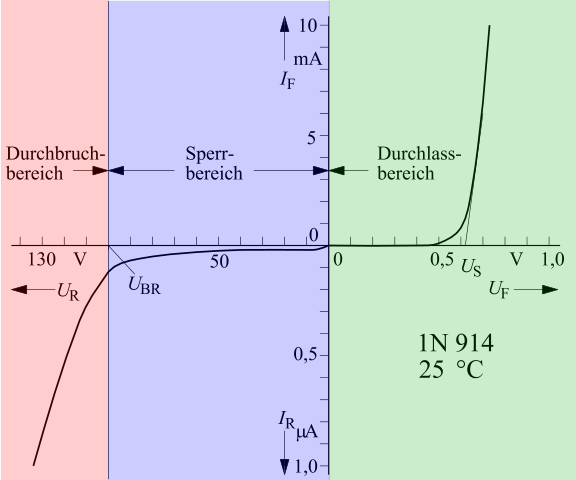
\includegraphics[scale=0.5]{Diode/Bilder/Kennlinie_Diode.png}
    \end{figure}
    }
\end{enumerate}

\mucho{8}{TC504}
{Eine in Sperrrichtung betriebene Diode hat}%Frage
{einen hohen Widerstand.}%A
{eine hohe Kapazität.}%B
{eine geringe Impedanz.}%C
{eine hohe Induktivität.}%D
{A}%Lösung

\mucho{9}{TC508}
{Wozu dient die folgende Schaltung?\\ 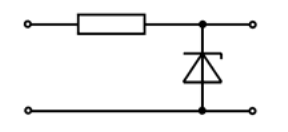
\includegraphics[scale=0.63]{Diode/Bilder/TC508.png}}%Frage
{zur Signalbegrenzung.}%A
{zur Spannungsstabilisierung.}%B
{als Leuchtanzeige.}%C
{zur Stromgewinnung.}%D
{B}%Lösung

\mucho{10}{TC505}
{Die Auswahlantworten enthalten Silizium-Dioden mit unterschiedlichen Arbeitspunkten. Bei welcher Antwort befindet sich die Diode in leitendem Zustand?}%Frage
{$-2,6V $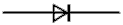
\includegraphics[scale=0.5]{Diode/Bilder/Diode_r.png} $-2,0V$}%A
{$~~~~15V$ 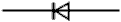
\includegraphics[scale=0.5]{Diode/Bilder/Diode_l.png} $~~~9V$}%B
{$~~0,7V$ 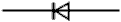
\includegraphics[scale=0.5]{Diode/Bilder/Diode_l.png} $1,3V$}%C
{$~~3,4V$ 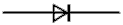
\includegraphics[scale=0.5]{Diode/Bilder/Diode_r.png} $4,0V$}%D
{C}%Lösung

\mucho{11}{TC506}
{Die Auswahlantworten enthalten Silizium-Dioden mit unterschiedlichen Arbeitspunkten. Bei welcher Antwort befindet sich die Diode in leitendem Zustand?}%Frage
{$~~5,3V $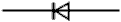
\includegraphics[scale=0.5]{Diode/Bilder/Diode_l.png} $4,7V$}%A
{$~~15V$ 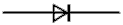
\includegraphics[scale=0.5]{Diode/Bilder/Diode_r.png} $18V$}%B
{$3,9V$ 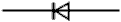
\includegraphics[scale=0.5]{Diode/Bilder/Diode_l.png} $3,2V$}%C
{$-2V$ 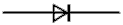
\includegraphics[scale=0.5]{Diode/Bilder/Diode_r.png} $-2,6V$}%D
{D}%Lösung

\mucho{12}{TC509}
{Wozu dient die folgende Schaltung?\\ 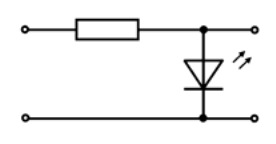
\includegraphics[scale=0.63]{Diode/Bilder/TC509.png}}%Frage
{zur Signalbegrenzung.}%A
{als Leuchtanzeige.}%B
{zur Stromgewinnung.}%C
{zur Spannungsstabilisierung.}%D
{B}%Lösung

\mucho{13}{TC507}
{Wie verhält sich die Kapazität einer Kapazitätsdiode (Varicap)?}%Frage
{Sie nimmt mit abnehmender Sperrspannung zu.}%A
{Sie erhöht sich mit zunehmender Durchlassspannung.}%B
{Sie nimmt mit zunehmender Sperrspannung zu.}%C
{Sie erhöht sich mit zunehmendem Durchlassstrom.}%D
{B}%Lösung


\chapter{Der Transistor}


\begin{wrapfigure}[2]{r}[-1cm]{4cm}
 \vspace{-6cm}
  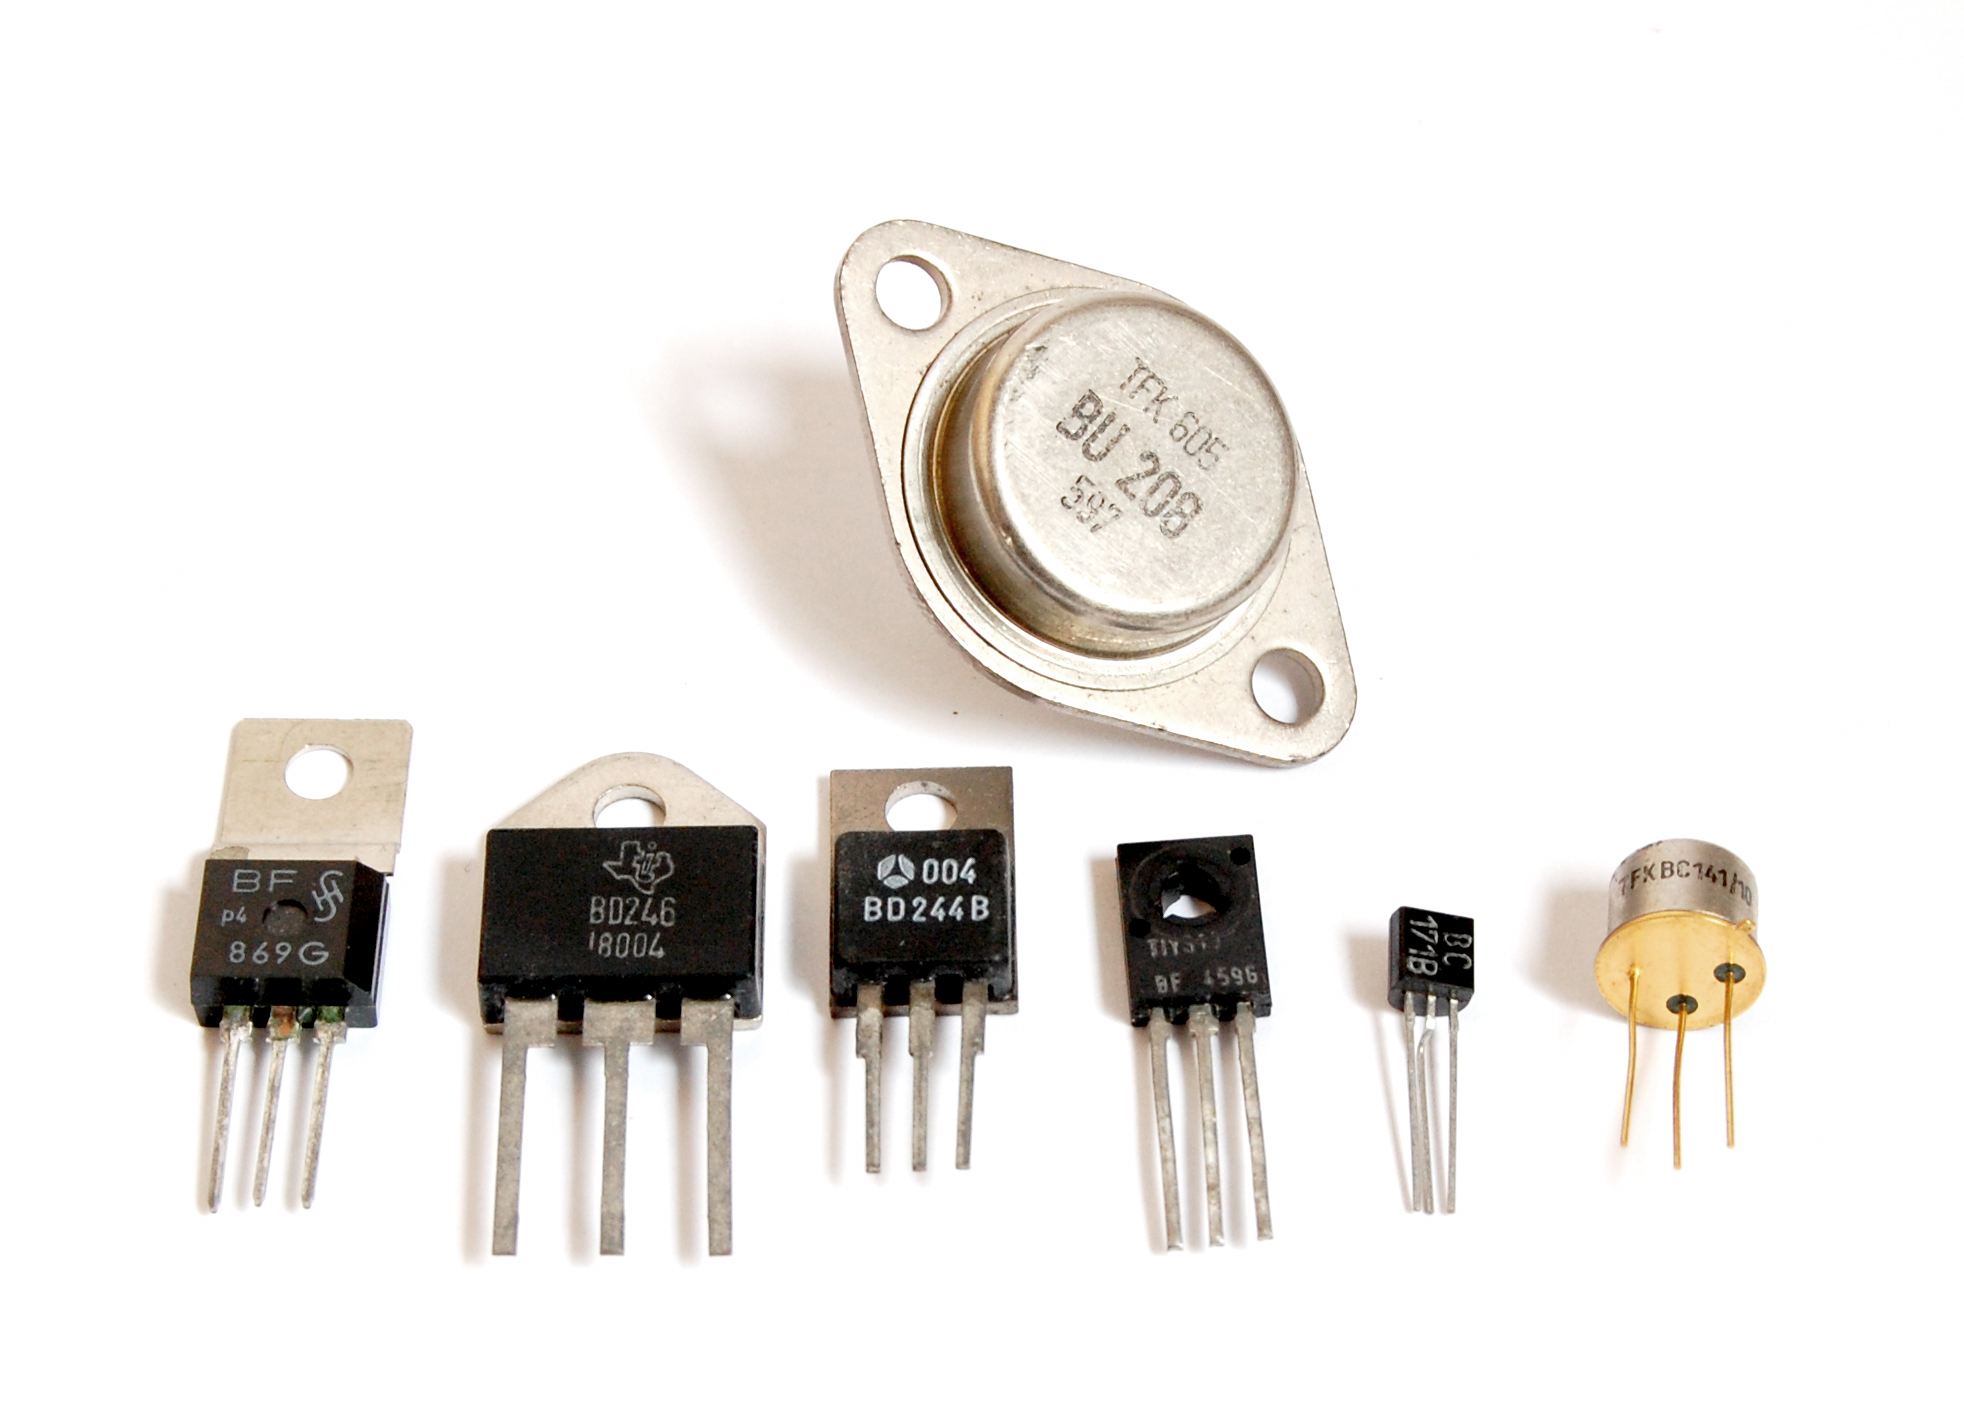
\includegraphics[scale=0.4]{Transistor/Bilder/Transistors-white.jpg}
 \vspace{-6cm}
\end{wrapfigure}

\section{Theorie- und Prüfungsfragen}

~~~~~~

\begin{enumerate}
\itemsep1pt\parskip0pt\parsep0pt
\item[i] Skizzieren Sie die Schaltzeichen eines NPN- und eines PNP-Transistors. Beschriften Sie entsprechend die Anschlüsse.
\item[ii] Zeichnen Sie das Ersatzschaltbild aus zwei Dioden für den NPN- und den PNP-Transistor.
\end{enumerate}

\begin{enumerate} 
\item[iii] \emph{\textbf{TC605}} Welche Kollektorspannungen haben NPN- und PNP-Transistoren?
	\begin{enumerate}
	\itemsep1pt\parskip0pt\parsep0pt
		\item[a] NPN- und PNP-Transistoren benötigen negative Kollektorspannungen.
		\item[b] PNP-Transistoren benötigen positive, NPN-Transistoren negative Kollektorspannung.
		\item[c] PNP- und NPN-Transistoren benötigen positive Kollektorspannungen.
		\item[d] NPN-Transistoren benötigen positive, PNP-Transistoren negative Kollektorspannungen.
	\end{enumerate}
\end{enumerate}

\loesung{	
	iii d
}

\begin{enumerate} 
\item[iv] \emph{\textbf{TC602}}  Das Verhältnis von Kollektorstrom zum Basisstrom eines Transistors liegt üblicherweise im Bereich von
	\begin{enumerate}
	\itemsep1pt\parskip0pt\parsep0pt
		\item[a] 1 zu 50 bis 1 zu 100.
		\item[b] 10 zu 1 bis 900 zu 1.
		\item[c] 1000 zu 1 bis 5000 zu 1.
		\item[d] 1 zu 100 bis 1 zu 500.
	\end{enumerate}
\end{enumerate}

\loesung{	
	iv b
}

\section{Praktische Anwendung}

\subsection[Der Bipolar-Transistor als Schalter]{Transistorschaltung 01 - Der Bipolar-Transistor als Schalter}

\begin{itemize}
\itemsep1pt\parskip0pt\parsep0pt
\item Schauen Sie sich den Bipolar-Transistor als Bauteil an und ordnen Sie die Bezeichnungen Kollektor, Basis und Emitter den einzelnen Beinchen zu.
\item Bauen Sie folgende Transistor-Schaltung auf (Abbildung \ref{s01}). 
\item Legen Sie die Versorgungsspannung an die Schaltung an.
\item Entfernen Sie unter Last die Leuchtdiode 1. Welche Auswirkungen hat das auf die Schaltung und warum?
\item \textbf{Zusatz:} Ersetzen Sie die Led durch einen Lautsprecher? Was passiert und warum?
\end{itemize}

\begin{figure}[H]
	\centering
	\subfigure[Schaltplan]{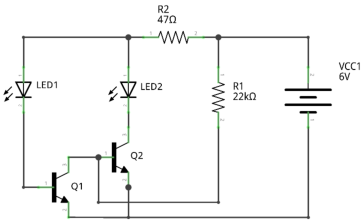
\includegraphics[scale=1.4]{Transistor/Schaltungen/NotBeleuchtung_Schaltplan.pdf}}
	\subfigure[Mögliche Breadboard-Ansicht]{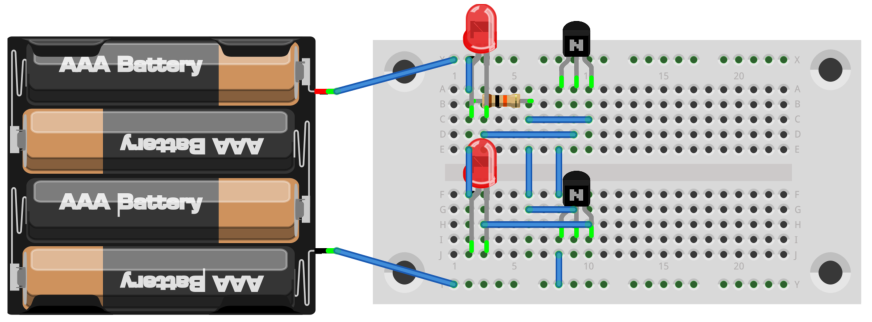
\includegraphics[scale=1]{Transistor/Schaltungen/NotBeleuchtung_Steckplatine.pdf}}
	\caption{Transistorschaltung 01 - Der Bipolar-Transistor als Schalter}
	\label{s01}
\end{figure}

%----------------------------------------------

\subsection[Der Bipolar-Transistor als Sensor]{Transistorschaltung 02 - Der Bipolar-Transistor als Sensor}

\begin{itemize}
\itemsep1pt\parskip0pt\parsep0pt
\item Bauen Sie folgende Transistor-Schaltung auf (Abbildung \ref{s02}). 
\item Legen Sie die Versorgungsspannung an die Schaltung an.
\item Berühren Sie die Basis des Transistors Q1 mit dem Finger. Was passiert und warum?
\end{itemize}

\begin{figure}[H]
	\centering
	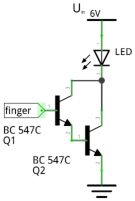
\includegraphics[scale=1.6]{Transistor/Schaltungen/NPN_Sensor.pdf}
	\caption{Transistorschaltung 02 - Der Bipolar-Transistor als Sensor}
	\label{s02}
\end{figure}

%----------------------------------------------

\subsection[Der Bipolar-Transistor als Verstärker]{Transistorschaltung 03 - Der Bipolar-Transistor als Verstärker}

\begin{itemize}
\itemsep1pt\parskip0pt\parsep0pt
\item Bauen Sie folgende Transistor-Schaltung auf (Abbildung \ref{s03}). 
\item Legen Sie die Versorgungsspannung an die Schaltung an.
\item Legen Sie ein Audiosignal an den Eingang der Schaltung an. Was passiert und warum?
\end{itemize}

\begin{figure}[H]
	\centering
	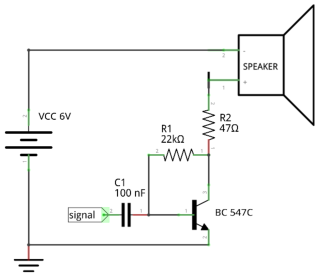
\includegraphics[scale=1.6]{Transistor/Schaltungen/NPN_Verstaerker.pdf}
	\caption{Transistorschaltung 03 - Der Bipolar-Transistor als Sensor}
	\label{s03}
\end{figure}

\chapter{Schwingkreis und Filter}
%\begin{wrapfigure}[0]{r}[-2.5cm]{3cm}
% \vspace{-6cm}
% \includegraphics[scale=0.4]{Schwingkreis/Bilder/schwingkreis.png}
% \vspace{-6cm}
%\end{wrapfigure}

\section*{Theorie- und Prüfungsfragen} 

\mucho{1}{TD203}
{Was ist im Resonanzfall bei der Reihenschaltung einer Induktivität mit einer Kapazität erfüllt?}%Frage
{Der Betrag des induktiven Widerstands ist dann gleich dem Betrag des kapazitiven Widerstands.}%A
{Der Wert des Verlustwiderstands der Spule ist dann gleich dem Wert des Verlustwiderstands des Kondensators.}%B
{Die Größe des elektrischen Feldes in der Spule ist dann gleich der Größe des elektrischen Feldes im Kondensators.}%C
{Die Größe des magnetischen Feldes in der Spule ist dann gleich der Größe des magnetischen Feldes im Kondensator.}%D
{A}%Lösung

\mucho{2}{TD209}
{Welche Resonanzfrequenz hat die Parallelschaltung einer Spule von 2 $\mu H$ mit einem Kondensator von 60 $pF$ und einem Widerstand von 10$k\Omega$?}%Frage
{145,288kHz}%A
{1,45288MHz}%B
{14,5288MHz}%C
{145,288 MHz}%D
{C \hspace{3em} $f_0 = \frac{1}{2 \pi \sqrt{L C}}$}%Lösung

\mucho{3}{TD206}
{ Wie ändert sich die Resonanzfrequenz eines Schwingkreises, wenn
1. die Spule mehr Windungen erhält, 2. die Länge der Spule durch Zusammenschieben der Drahtwicklung verringert wird, 3. ein Kupferkern in das Innere der Spule gebracht wird?}%Frage
{Die Resonanzfrequenz wird bei 1. und 2. kleiner und bei 3. größer.}%A
{Die Resonanzfrequenz wird in allen drei Fällen kleiner.}%B
{Die Resonanzfrequenz wird bei 1. kleiner und bei 2. und 3. größer.}%C
{Die Resonanzfrequenz wird bei 1. und 2. größer und bei 3. kleiner.}%D
{A}%Lösung


\mucho{4}{TD201}
{Der Impedanzfrequenzgang in der Abbildung zeigt die Kennlinie\\ 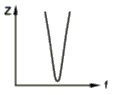
\includegraphics[scale=0.5]{Schwingkreis/Bilder/TD201.png}}%Frage
{eines Serienschwingkreises.}%A
{eines Parallelschwingkreises.}%B
{einer Induktivität.}%C
{einer Kapazität.}%D
{A}%Lösung

\vspace*{0.65cm}

\mucho{5}{TD202}
{Der Impedanzfrequenzgang in der Abbildung zeigt die Kennlinie\\
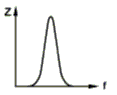
\includegraphics[scale=0.5]{Schwingkreis/Bilder/TD202.png}}%Frage
{eines Serienschwingkreises.}%A
{eines Parallelschwingkreises.}%B
{einer Induktivität.}%C
{einer Kapazität.}
{B}%Lösung

\aufgabentext{
	\begin{enumerate}
	\item[6] Um welche Schaltungen handelt es sich in folgender Abbildung.
	\end{enumerate}
	\loesung{1 Reihenschwingkreis, 2 Parallelschwingkreis, 3 Tiefpass, 4 Hochpass, 5 Bandpass, 6 Saugkreis, 7 Sperrkreis }
	}

\begin{figure}[H]
	\centering
	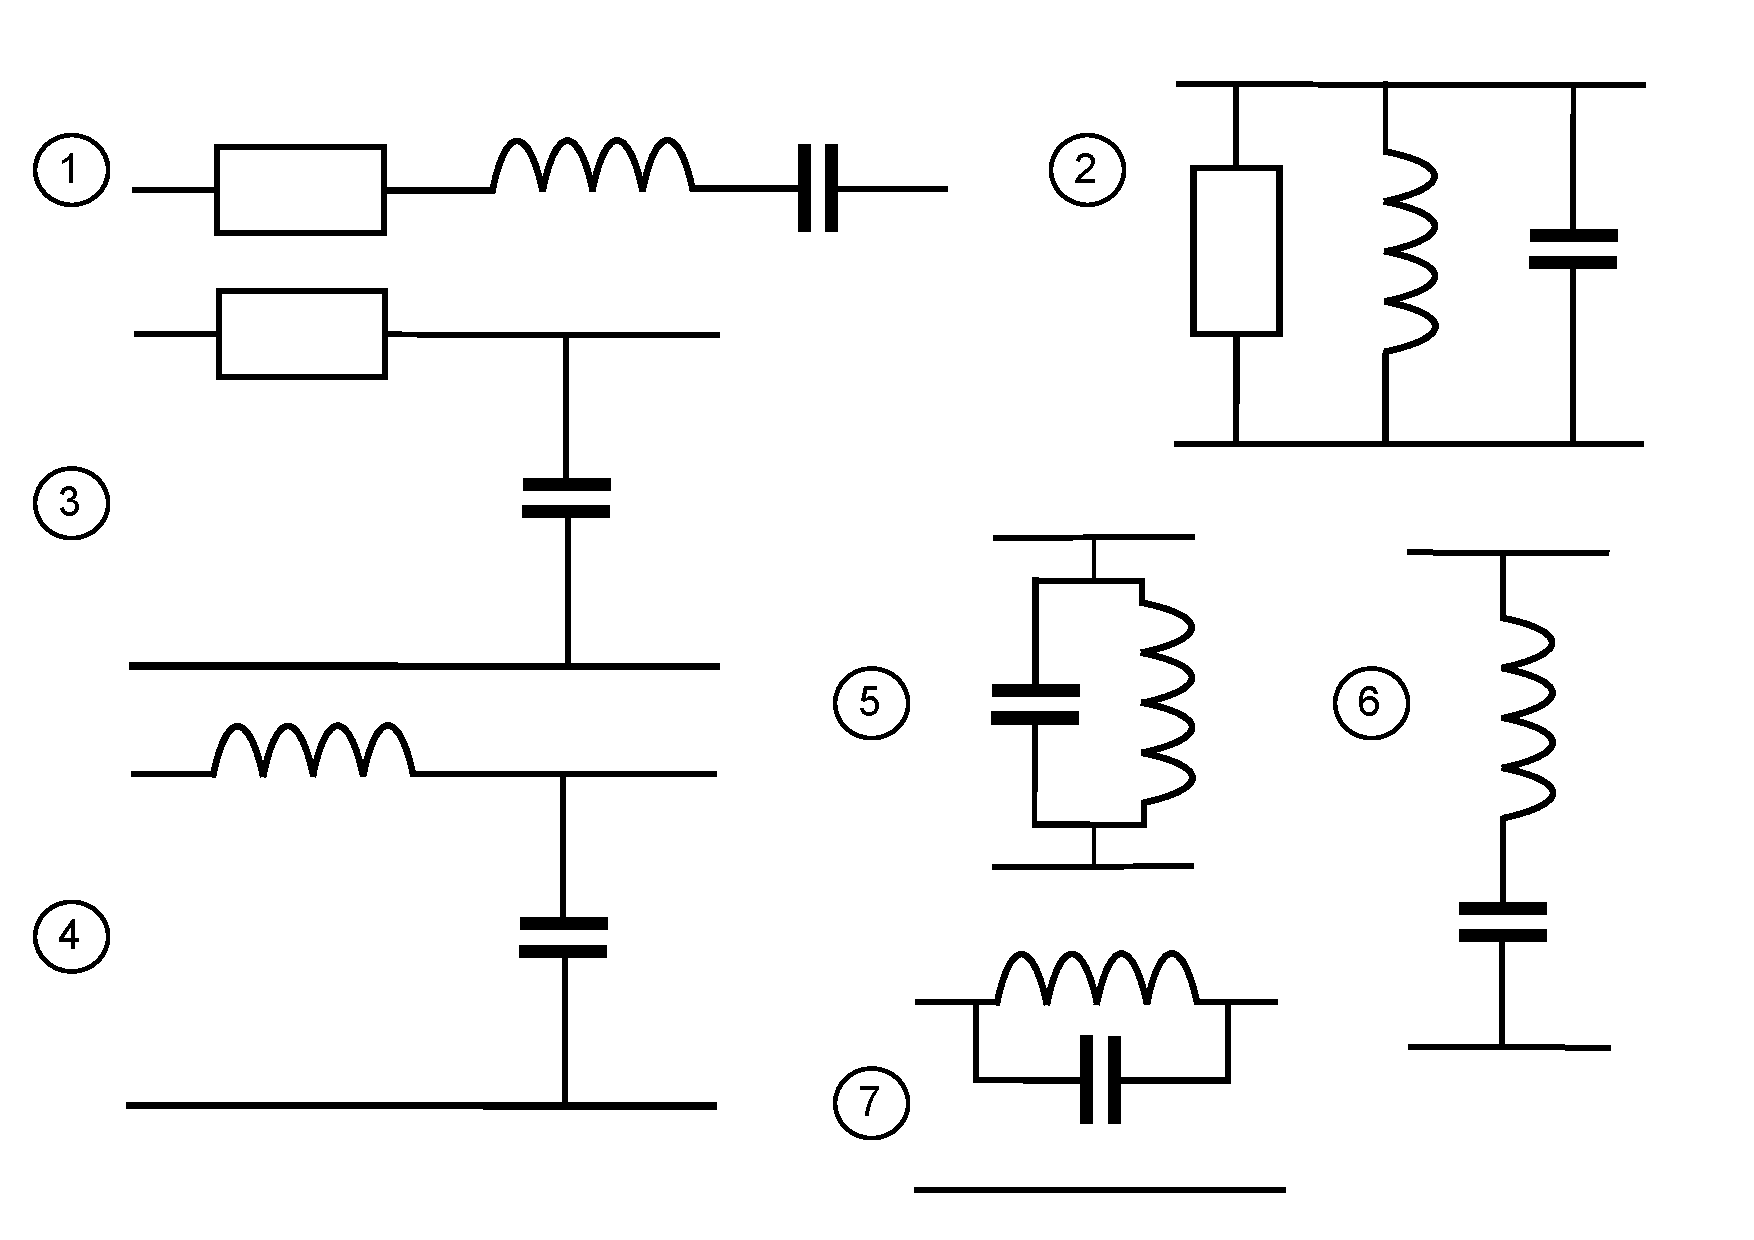
\includegraphics[scale=0.5]{Schwingkreis/Bilder/Filterschaltungen.pdf}
	\end{figure}

\mucho{7}{TD213}
{Welche Grenzfrequenz ergibt sich bei einem RC-Tiefpass mit einem Widerstand von 10$k\Omega$ und einem Kondensator von 50$nF$?}%Frage
{0,32$Hz$}%A
{318$Hz$}%B
{421$Hz$}%C
{318$kHz$}%D
{B \hspace{3em} $f_g = \frac{1}{2 \pi R C}$}%Lösung

\section*{Praxis}

\subsection*{Vorbereitung}

Seht euch die Pin-Belegung des Raspberry Pi (siehe Abbildung \ref{rpi}) sowie
die zu layoutende Schaltung für den 70cm-Tiefpassfilter (siehe Abbildung
\ref{70cmLP}) an.

\begin{figure}[H]
    \centering
    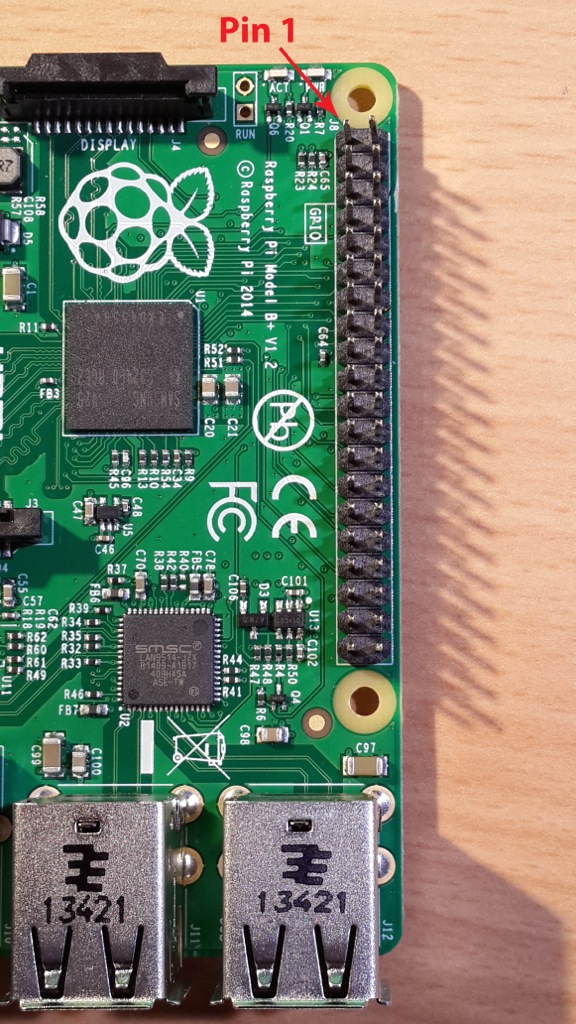
\includegraphics[height=0.4\textheight]{Schwingkreis/Bilder/B_plus_hdr_sm.jpg}
    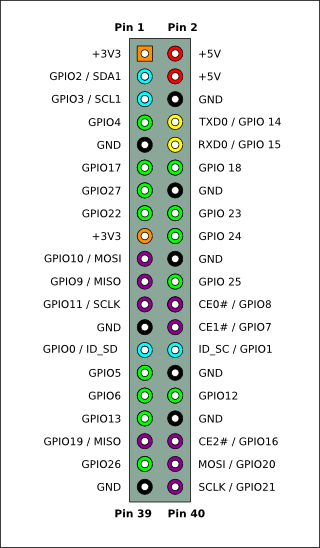
\includegraphics[height=0.4\textheight]{Schwingkreis/Bilder/Pi-GPIO-header.png}
    \caption{Connector pinout (P1 Header) -- Models B+, B2}
    \label{rpi}
    %FIXME Abbildungs-Quellenverzeichnis \url{http://elinux.org/RPi_Low-level_peripherals#Model_A.2B.2C_B.2B_and_B2}
\end{figure}

\begin{figure}[H]
    \centering
    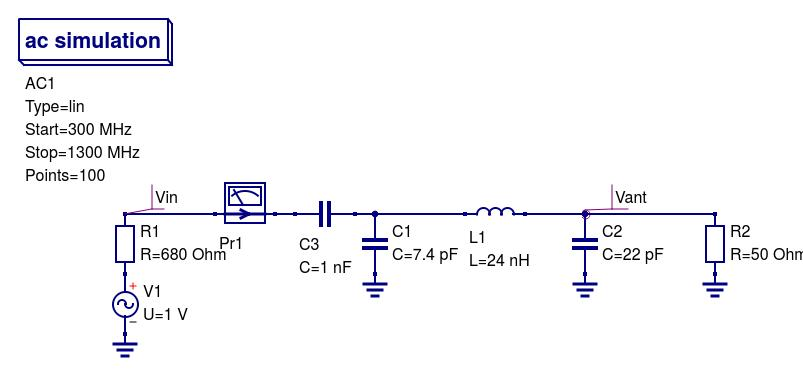
\includegraphics[width=1\textwidth]{Schwingkreis/Bilder/70cmLP500Ohm.jpg}
    \caption{Schaltung des 70cm-Tiefpassfilters aus Qucs}
    \label{70cmLP}
\end{figure}

\subsection*{Fritzing}

\subsubsection{Schematic View}

Bauteile aus den \emph{Core Parts} hinzufügen:

\begin{itemize}
    \item  Basic
    \begin{itemize}
        \item Resistor $680 \Omega$ (THT)
        \item Inductor $22 nH$ (SMD 1206)
        \item Ceramic Capacitor $1 nF$ (THT)
        \item Ceramic Capacitor $22 pF$ (THT)
    \end{itemize}
    \item  Input
    \begin{itemize}
        \item Variable Capacitor $2.1-10 pF$ (THT, $3.81mm$ pin spacing)
        \item Antenna (Wire soldering point)
    \end{itemize}
    \item Connection
    \begin{itemize}
        \item Generic female header (THT, 2x10, flip horizontal)
    \end{itemize}
    \item Schematic View
    \begin{itemize}
        \item Ground
    \end{itemize}
\end{itemize}

Nun können die Bauteile entsprechend des Schaltplanes verdrahtet werden.
\textbf{Hinweis}: Die Pin-Zählung des \emph{Generic female header} stimmt nicht
mit der des Raspberry Pi überein.

\begin{itemize}
    \item GPIO = Pin 16
    \item GND = Pin 17
\end{itemize}

\subsubsection{PCB View}

\begin{itemize}
    \item PCB ändern auf One Layer \& Fäche ca. $30x30mm$
    \item Bauteile anordnen (THT-Bauteile auf Vorderseite, SMD auf Unterseite)
    \item Leitungen ziehen
    \item optional: Copper Fill Blocker \& Silkscreen Text
    \item Rechtsklick auf einen Ground Pin: "`Set Ground Fill Seed"'
    \item Menü $\rightarrow$ Routing $\rightarrow$ Ground Fill
\end{itemize}

\subsubsection{Zusatzaufgaben}

\begin{itemize}
    \item Antennenanschluss auf folgende MCX-Buchse umbauen: \\
          \url{http://www.reichelt.de/index.html?ARTICLE=152523}
    \item Testboard mit verschiedenen PCB-Spulen um ~24 nH erstellen, da typ. 2-3\% Abweichung. \\
          Berechnungsgrundlagen mit Online calculator:\\
          \url{http://coil32.net/pcb-coil.html}\\
          alternative Formen: \\
          \url{http://www.circuits.dk/calculator_planar_coil_inductor.htm}
\end{itemize}


% Literaturverzeichnis
\bibliographystyle{natdin}
\addcontentsline{toc}{section}{Literaturverzeichnis}
\bibliography{Literaturverzeichnis}
% Abbildungsverzeichnis
\newpage
\addcontentsline{toc}{section}{Abbildungsverzeichnis}
\listoffigures	
%Anhang

\end{document}


